\documentclass[a4paper,12pt]{article}
\usepackage[utf8]{inputenc}
\usepackage[T2A]{fontenc}
\usepackage[russian]{babel}
\usepackage{graphicx}
\usepackage{setspace}
\usepackage{geometry}
\geometry{left=2cm, right=2cm, top=2cm, bottom=2cm}
\usepackage{parskip} % для удобного разделения абзацев
\usepackage{xcolor}
\usepackage{hyperref}
\usepackage{listings}

\usepackage{newunicodechar}
\newunicodechar{└}{\texttt{+}}
\newunicodechar{├}{\texttt{+}}
\newunicodechar{─}{-}
\newunicodechar{│}{|}


\lstset{
    basicstyle=\ttfamily\small,
    frame=single,
    backgroundcolor=\color{lightgray!20},
    breaklines=true,
    columns=fullflexible,
    language=sh,
    extendedchars=false
}


% Настройка стиля ссылок
\hypersetup{
    colorlinks=true,
    linkcolor=black,      % Цвет внутренних ссылок
    citecolor=black,      % Цвет библиографических ссылок
    urlcolor=blue         % Цвет гиперссылок (тёмно-голубой/бирюзовый)
}

\newcommand{\customlink}[2]{\textit{\href{#1}{#2}}} % Создаём макрос для ссылок в курcиве
\begin{document}

% Титульный лист
\begin{titlepage}
    % Верхняя часть: логотип, название олимпиады и проекта, выровнено по центру
    \begin{center}
        
\includegraphics[width=0.3\textwidth]{../Include/logo.png}\\[1cm]

        {\itshape\Large\bfseries Студенческая олимпиада «Газпром» - конкурс проектов\par}
        \vspace{0.5cm}

        {\Large\bfseries Пояснительная записка к проекту\par}
        \vspace{2cm}

        {\large Название конкурсного проекта: \par}
        \vspace{0.3cm}

        {\LARGE\bfseries Прогнозирование отказов оборудования и аварийных ситуаций в газовой и нефтяной промышленности\par}
        \vspace{0.5cm}

    \end{center}

    % Нижняя часть: информация об авторе, вузах, ключевых словах, выровнена по левому краю и меньшим шрифтом
    \begin{flushleft}
        {\normalsize
        \textbf{Выполнил:} Мурадян Денис Степанович\par
        \vspace{0.3cm}
        \textbf{Вуз участника:} Санкт-Петербургский государственный университет\par
        \vspace{0.3cm}
        \textbf{Вуз, на площадке которого планируется защита:} \par
        Санкт-Петербургский государственный электротехнический университет «ЛЭТИ» им. В.И. Ульянова (Ленина)\par
        \vspace{0.3cm}
        \textbf{Ключевые слова:} искусственный интеллект, прогнозирование отказов, мониторинг оборудования, безопасность,
            GRU, RNN, AI, нефтегазовая промышленность, интеллектуальный анализ данных, анализ данных, аварийные ситуации\par
        \textbf{Контактная информация:}\par
        \quad Почта: \href{mailto:muradyan.denis@inbox.ru}{muradyan.denis@inbox.ru}\par
        \quad Telegram: \href{https://t.me/DenisMuradyan}{@DenisMuradyan}\par
        }
    \end{flushleft}

\end{titlepage}

\newpage
\tableofcontents
\newpage

\newpage
\section{\centering Аннотация}

\begin{flushleft}
Проект предназначен для повышения безопасности и эффективности эксплуатации оборудования в газовой и нефтяной промышленности
посредством интеллектуального мониторинга. В основе решения лежит нейронная сеть, которая осуществляет непрерывный анализ данных,
поступающих с датчиков, и предсказывает вероятность отказа оборудования в режиме реального времени.

Этот подход позволяет своевременно выявлять потенциальные угрозы, оптимизировать процессы технического
обслуживания и снижать финансовые потери, связанные с аварийными ситуациями.
Высокая точность предсказаний нейронной сети является ключевой особенностью проекта,
обеспечивая надежное и оперативное реагирование на изменения в состоянии оборудования.

Кроме того, предоставляется возможность запуска сервера-мониторинга онлайн, что позволяет наблюдать за
предсказаниями модели из любой точки мира, имея доступ в интернет.
Это обеспечивает удобство и оперативность мониторинга, способствуя принятию обоснованных решений операторами и инженерами.

Решение, основанное на современных технологиях машинного обучения, демонстрирует высокий научно-технический потенциал
и соответствует актуальным требованиям нефтегазовой отрасли.
Проект будет особенно полезен для компании Газпром, так как позволяет существенно снизить эксплуатационные риски,
оптимизировать затраты на техническое обслуживание и ремонт, а также повысить надежность работы оборудования.
Целевая аудитория проекта включает операторов, инженеров, руководителей и специалистов по эксплуатации и инновациям.
\end{flushleft}


\newpage
\section{Выявление проблемы и постановка задач проекта}
\begin{flushleft}
В современном мире обеспечение безопасности и надежности эксплуатации оборудования в газовой и
нефтяной промышленности является одним из ключевых факторов стабильного функционирования энергетической инфраструктуры.
С каждым годом растут требования к техническому состоянию объектов, а также к оперативности реагирования на непредвиденные ситуации.
Отсутствие эффективных систем раннего предупреждения может привести к возникновению аварий,
последствия которых оказываются катастрофическими для экономики, экологии и человеческих жизней.

\subsection{Статистические данные и исторические примеры: }
В последние годы в нефтегазовой отрасли, зафиксированы серьёзные аварийные инциденты,
имеющие как экономические, так и социальные и экологические последствия.
Так, в декабре 2022 года на магистральном газопроводе «Уренгой-Помары–Ужгород» произошёл взрыв, причиной которого стала утечка газа.
В результате которого погибли три человека и произошла временная остановка транзитных поставок
(см. \href{https://oilcapital.ru/news/2022-12-23/gazoprovody-pod-udarom-2623441}{источник}).
В августе 2021 года пожар на заводе «Газпрома» в Новом Уренгое привёл к значительным экономическим потерям
и снижению объёмов прокачки газа (см. \href{https://www.rbc.ru/business/06/08/2021/610d06959a7947180b906801}{источник}).
Аналогичные последствия имела разгерметизация подземного газопровода в Санкт-Петербурге в октябре 2022 года,
а разрыв магистрального газопровода «Белоусово– Ленинград» в Ленинградской области в ноябре 2022 года привёл
к отключению нескольких газораспределительных станций
(см. \href{https://oilcapital.ru/news/2022-12-23/gazoprovody-pod-udarom-2623441}{источник}).
Кроме того, аварии на объекте ООО «Газпром трансгаз Екатеринбург» в 2021 году сопровождались утечками газа,
что усугубило экологическую ситуацию
(см. \href{https://www.gazprom.ru/f/posts/57/982072/gazprom-environmental-report-2021-ru.pdf}{источник}).

\subsection{Выявление проблемы: }

Эти примеры наглядно демонстрируют, что аварийность в нефтегазовой отрасли остаётся высокой,
а последствия таких инцидентов – разрушительными.
Каждая авария сопровождается значительными убытками, утратой человеческих жизней, ухудшением экологической обстановки
и финансовыми потерями, что подчеркивает необходимость разработки эффективных мер по их предотвращению.

Исходя из вышеизложенного, можно сделать вывод, что отсутствие эффективных систем раннего
обнаружения отказа оборудования приводит к аварийным ситуациям с серьёзными последствиями
для экономики, экологии и безопасности людей.
Это подчёркивает острую необходимость разработки современного инструмента,
который позволит заблаговременно выявлять потенциальные угрозы и предупреждать об аварийных ситуациях.

\subsection{Цель и задачи: }

Таким образом, основная цель проекта заключается в создании системы,
способной заблаговременно выявлять потенциальные угрозы и предупреждать об аварийных ситуациях.

Для её реализации в рамках проекта поставлены следующие задачи:
\begin{itemize}
    \item Разработать систему, способную прогнозировать отказы оборудования с высокой точностью;
    \item Обеспечить анализ потоковых данных в режиме реального времени для оперативного выявления потенциальных угроз;
    \item Интегрировать передовые решения, такие как искусственный интеллект, для детального анализа временных последовательностей данных с датчиков;
    \item Разработать REST API для оперативного обмена информацией между системой мониторинга и пользователями;
    \item Обеспечить возможность удалённого мониторинга через интернет;
\end{itemize}
\end{flushleft}





\section{Техническое описание решения}
\begin{flushleft}

В данном разделе описываются основные технические решения проекта, позволяющие обеспечить высокую точность прогнозирования отказов оборудования и оперативный доступ к к этим прогнозам.

\subsection{Архитектура системы}
Проект представляет собой модульную систему, составленную из следующих основных компонентов. Ниже приведена структура каталогов с краткими комментариями:

\lstset{
    basicstyle=\ttfamily\small,
    frame=single,
    backgroundcolor=\color{lightgray!20},
    breaklines=true,
    columns=fullflexible,
    language=sh,
    extendedchars=false
}

\begin{lstlisting}
Project/
├── app/
│   ├── __init__.py
│   ├── main.py               # Серверное приложение на базе FastAPI, реализующее REST API и дашборд
│   ├── inference.py          # Функции предобработки данных и вызова модели
│   └── dashboard.html        # HTML-страница для визуального контроля показателей риска
├── data/
│   ├── generate_dataset.py   # Формирует синтетический датасет и имитирует поступление данных
│   ├── sensor_train_data.csv # Датасет для обучения модели
│   ├── sensor_val_data.csv   # Датасет для валидации модели
│   └── sensor_test_data.csv  # Датасет для тестирования модели
├── model/
│   ├── __init__.py
│   ├── model.py              # Подготовка данных, обучение GRU модели, логирование
│   ├── logs/
│   │   ├── total_log.txt     # Информация о модели и отслеживаемых параметрах
│   │   └── training_log.csv  # Метрики на каждой эпохе обучения
│   └── saved_models/
│       └── gru_model.h5      # Сохранённая обученная модель
├── simulation_data/
│   └── data_simulator.py     # Скрипт для симуляции поступления данных в реальном времени
└── README.md                 # Документация проекта
\end{lstlisting}

\noindent
Каждый каталог содержит файлы и скрипты, отвечающие за свою часть функционала:
\begin{itemize}
    \item \textbf{app/} --- серверное приложение на базе FastAPI (REST API, дашборд).
    \item \textbf{data/} --- генерация и хранение датасетов для обучения, валидации и тестирования модели.
    \item \textbf{model/} --- подготовка данных, обучение GRU-модели, логирование результатов.
    \item \textbf{simulation\_data/} --- инструменты для имитации поступления данных в режиме реального времени.
\end{itemize}


\subsection{Принцип работы системы}

Система функционирует поэтапно, обеспечивая непрерывный мониторинг и предсказание отказов оборудования в режиме реального времени:

\begin{enumerate}
    \item \textbf{Получение данных.}
    Поток данных поступает от датчиков в реальном времени. Для демонстрационных целей используется синтетическая генерация, реализованная в \texttt{generate\_dataset.py}, который подготавливает обучающий, валидационный и тестовый датасеты. Скрипт \texttt{data\_simulator.py} имитирует поступление данных от датчиков для проверки работы системы.

    \item \textbf{Обработка данных.}
    Все входные данные нормализуются и приводятся к необходимому формату в модуле \texttt{inference.py}. После предобработки данные передаются на вход обученной модели.

    \item \textbf{Предсказание отказа.}
    На основе 20 последовательных отсчётов (каждый содержит 5 параметров от датчиков) обученная GRU-модель оценивает вероятность отказа оборудования. Число в 20 отсчётов выбрано эмпирически для сохранения контекста работы установки и более точного прогнозирования.

    \item \textbf{Доступ к результатам.}
    Серверное приложение, запущенное в \texttt{app/main.py}, предоставляет REST API для получения предсказаний. Также доступен дашборд, где в режиме реального времени можно контролировать уровень риска для каждого объекта. Это позволяет оперативно реагировать на возможные проблемы и принимать обоснованные решения по профилактике и обслуживанию оборудования.
\end{enumerate}

\subsubsection{Основные модули и их роль}

\begin{itemize}
    \item \textbf{app/main.py} \\
    Запускает сервер FastAPI, загружает сохранённую модель и предоставляет следующие эндпоинты REST API:
    \begin{itemize}
        \item \texttt{/predict}: принимает последовательность данных с датчиков и возвращает рассчитанную вероятность отказа.
        \item \texttt{/update} и \texttt{/predictions}: обновляют и хранят последние предсказания для каждой установки.
        \item \texttt{/dashboard}: отдает HTML-страницу для визуального контроля показателей риска отказа.
    \end{itemize}

    \item \textbf{app/inference.py} \\
    Содержит функции для нормализации входных данных и выполнения предсказания модели.

    \item \textbf{data/generate\_dataset.py} \\
    Формирует синтетический датасет, имитируя поступление данных с датчиков. Для каждой из 10 установок задаются базовые параметры (давление, температура, вибрация, расход газа), которые затем изменяются под воздействием случайных колебаний и событий, имитирующих начало отказа.

    \item \textbf{model/model.py} \\
    Отвечает за:
    \begin{itemize}
        \item Формирование последовательностей данных и разметку сценариев отказа;
        \item Построение GRU-модели для бинарной классификации (отказ/без отказа);
        \item Обучение модели с логированием основной информации об обучении в файлы \texttt{total\_log.txt} и \texttt{training\_log.csv}, которые находятся в каталоге \texttt{model/logs}.
    \end{itemize}

    \item \textbf{simulation\_data/data\_simulator.py} \\
    Имитирует поток данных, формируемых на основе датасета, и отправляет их на сервер для демонстрации работы системы в условиях, приближенных к реальным.
\end{itemize}

\subsection{Датасет}

\subsubsection{Структура и формирование данных}

Датасет формируется с помощью скрипта \texttt{generate\_dataset.py} и используется для обучения, валидации модели, а также демонстрации работоспособности системы. Каждая запись датасета содержит следующие признаки:
\begin{itemize}
    \item \textbf{timestamp:} Временная метка (например, \texttt{2025-03-15 11:00:01}).
    \item \textbf{segment\_id:} Идентификатор установки (например, A1, A2, \dots, A10).
    \item \textbf{pressure:} Давление, исходные значения которого составляют примерно 7.0--9.0 bar с постепенными изменениями.
    \item \textbf{temperature:} Температура, начальные значения варьируются в пределах 20.0--25.0\,°C.
    \item \textbf{vibration:} Уровень вибрации, исходные значения составляют около 0.03--0.07 м/с.
    \item \textbf{flow\_rate:} Расход газа, начальные значения находятся в диапазоне 150.0--250.0 м³/час.
\end{itemize}

\subsubsection{Принцип формирования данных}

Датасет создаётся с учетом двух ключевых режимов:
\begin{enumerate}
    \item \textbf{Нормальные условия работы.} \\
    Для каждой установки задаются базовые значения параметров, которые затем подвергаются естественному дрейфу и случайным колебаниям для имитации реальной работы оборудования.

    \item \textbf{Симуляция отказа.} \\
    Для отдельных установок в случайный момент запускается сценарий (симуляция аварийных ситуаций), имитирующий начало отказа. Это может выражаться в резком изменении давления, уменьшении пропускаемости, последовательном повышении температуры или вибрации. При этом вероятность отказа крайне низкая (около 0.5\%), что подчеркивает важность обнаружения даже единичных случаев. Из 10\,000 нормальных показаний критически важно зафиксировать хотя бы один отказ.
\end{enumerate}

\noindent На основании изменений параметров системе присваивается метка риска отказа, что позволяет операторам своевременно принимать меры по профилактике.


    \subsection{Создание и обучение модели}

\subsubsection{Выбор архитектуры}

В задачах анализа данных с датчиков, где измерения производятся каждую секунду, крайне важно учитывать временные взаимосвязи между последовательными наблюдениями. При работе с такими данными традиционные модели, например, MLP (Multi-Layer Perceptron), не справляются с захватом динамики изменений, поскольку они обрабатывают данные последовательно, независимо от предыдущих показаний.

Рекуррентные нейронные сети (RNN – Recurrent Neural Network) специально созданы для анализа последовательных данных. Они обрабатывают следующие данные на основе уже обработанных, что делает их более подходящими для решения подобных задач. Однако классические RNN страдают от проблемы затухания и взрыва градиента, особенно при обработке длинных последовательностей, что затрудняет обучение модели.

В связи с этим была выбрана архитектура GRU (Gated Recurrent Unit) --- усовершенствованная версия RNN, которая благодаря внутренним механизмам управления потоком данных частично решает проблему затухания и взрыва градиента. GRU-модель эффективна при обработке временных рядов, поскольку способна сохранять и использовать информацию о прошлых наблюдениях, что особенно важно при анализе последовательных данных с датчиков.

\subsubsection{Сценарии отказа}

В процессе подготовки данных в модуле \texttt{model/model.py} реализованы следующие сценарии, указывающие на риск отказа:
\begin{itemize}
    \item Резкое увеличение давления на протяжении последовательности (рост более 20\%);
    \item Последовательное повышение температуры в условиях устойчиво высокого давления;
    \item Сохранение высокого уровня давления при снижении расхода газа;
    \item Сочетание постоянного высокого уровня вибрации с непрерывным ростом температуры;
    \item Дополнительные эвристические условия, учитывающие экстремальные значения отдельных параметров.
\end{itemize}

\subsubsection{Логирование}

Основная информация об обучении модели фиксируется в файлах, расположенных в каталоге \texttt{model/logs}:
\begin{itemize}
    \item \texttt{total\_log.txt} --- информация о модели и отслеживаемых параметрах;
    \item \texttt{training\_log.csv} --- информация о параметрах в каждой эпохе.
\end{itemize}
В этих файлах сохраняются данные о модели, отслеживаемых параметрах, использовании памяти и времени тренировки.

\subsubsection{Настройка гиперпараметров}

Настройка гиперпараметров представлена ниже:
\begin{lstlisting}
Loss function: Focal Loss для бинарной классификации
Count layers: 2
Count neurons: [64, 32]
Metrics: Accuracy, AUC, Precision, Recall
Count epochs: 50
\end{lstlisting}

\subsubsection{Результаты обучения}

Ниже приведены ключевые показатели, полученные в ходе обучения модели:
\begin{lstlisting}
Type: GRU-based RNN (Sequential model)
Count layers: 2
Count neurons: [64, 32]
Loss function: <function focal_loss.<locals>.focal_loss_fixed at 0x000001C9299CEE80>
Count epochs: 50
Metrics: accuracy, <AUC name=auc>, <Precision name=precision>, <Recall name=recall>
Memory used during training: 512.71 MB
Total training time: 190.22 seconds

Baseline metrics:
Loss before training (Train): 0.0440
Loss before training (Validation): 0.0440

Final metrics:
Loss after training (Train): 0.0113
Loss after training (Validation): 0.0113
Training metrics: loss = 0.0113, accuracy = 0.9125, auc = 0.9777, precision = 0.8490, recall = 0.9178
Validation metrics: loss = 0.0113, accuracy = 0.9125, auc = 0.9777, precision = 0.8490, recall = 0.9178
\end{lstlisting}

\subsubsection{Интерпретация результатов}

В ходе обучения GRU-модели для прогнозирования отказов оборудования получены следующие ключевые метрики, позволяющие оценить качество и надежность решения:
\begin{itemize}
    \item \textbf{Loss (Потери):} Значение функции потерь снизилось с 0.0440 до 0.0113 как на обучающей, так и на валидационной выборках. Это свидетельствует о том, что модель хорошо подстроилась под данные и её предсказания максимально приближены к истинным меткам. Низкое значение loss особенно важно для обнаружения редких событий, таких как отказ оборудования.
    \item \textbf{Accuracy (Точность):} Достигнутая точность в 91.25\% указывает на то, что в 91 из 100 случаев модель верно классифицирует состояние оборудования. Такая стабильность подтверждает, что модель способна различать нормальное состояние и потенциальные сбои, что критично для своевременного принятия мер.
    \item \textbf{AUC (Площадь под ROC-кривой):} Значение AUC равное 0.9777 демонстрирует отличную способность модели различать между классами «отказ» и «без отказа». Высокий AUC особенно важен при работе с несбалансированными данными, где позитивные случаи встречаются редко.
    \item \textbf{Precision (Точность предсказаний отказов):} Precision на уровне 84.90\% указывает, что из всех предсказанных отказов около 85\% действительно соответствуют реальным отказам, что снижает вероятность ложных тревог и оптимизирует процессы профилактического обслуживания.
    \item \textbf{Recall (Полнота обнаружения отказов):} Значение recall на уровне 91.78\% демонстрирует высокую чувствительность модели, позволяющую обнаружить большинство реальных случаев отказа. Это особенно важно в задачах, где пропуск отказа может привести к аварийной ситуации.
\end{itemize}

Примеры работы модели:
\begin{itemize}
    \item При анализе последовательностей с постепенным повышением температуры и резким скачком давления, модель демонстрирует высокую уверенность в прогнозе отказа, что позволяет оперативно проводить мероприятия по предотвращению аварий.
    \item В сценариях, когда изменения параметров менее выражены, но наблюдается устойчивая тенденция к ухудшению показателей, высокая чувствительность (recall) модели помогает выявить потенциально опасные отклонения на ранней стадии.
    \item Снижение количества ложноположительных срабатываний, подтвержденное значением precision, свидетельствует о том, что модель не склонна к чрезмерным срабатываниям, что важно для рационального распределения ресурсов на проверку оборудования.
\end{itemize}

Таким образом, полученные метрики свидетельствуют о том, что модель надёжно различает исправное состояние оборудования и потенциальный отказ, что подтверждает её пригодность для практического применения и позволяет оперативно реагировать на критические ситуации, повышая безопасность и снижая эксплуатационные риски.


    \subsection{Получение и обработка данных}

\subsubsection{REST API}

Серверное приложение в \texttt{app/main.py} предоставляет REST API для решения следующих задач:
\begin{itemize}
    \item Приём данных с датчиков через POST-запросы на эндпоинт \texttt{/predict};
    \item Обновление и хранение последних предсказаний через эндпоинты \texttt{/update} и \texttt{/predictions};
    \item Отдача HTML-дашборда на эндпоинте \texttt{/dashboard} для визуального контроля показателей риска.
\end{itemize}

\subsubsection{Симуляция данных}

Скрипт \texttt{simulation\_data/data\_simulator.py} формирует данные из датасета, имитируя поток информации, поступающий от датчиков в реальном времени. Полученные данные отправляются на сервер, который обрабатывает их и возвращает предсказания вероятности отказа. Это позволяет проверить работоспособность системы в условиях, приближенных к реальным.

\subsection{Настройка и запуск проекта}

\subsubsection{Требования}

\begin{itemize}
    \item \textbf{Python 3.11} – убедитесь, что установлен Python указанной версии или выше.
    \item \textbf{requirements} – установите необходимые зависимости:
\begin{lstlisting}[%
  basicstyle=\ttfamily\small,
  frame=single,
  backgroundcolor=\color{lightgray!20},
  breaklines=true,
  columns=fullflexible,
  language=sh,
  extendedchars=false
]
pip install -r requirements.txt
\end{lstlisting}
    \item \textbf{Node.js} – необходим для онлайн-запуска с LocalTunnel. Скачайте и установите с \href{https://nodejs.org/}{официального сайта}.
\end{itemize}

\subsubsection{Запуск проекта}

Проект может быть запущен двумя способами: локально или с помощью LocalTunnel, чтобы предоставить доступ к серверу из интернета.

\paragraph{1. Локальный запуск}

\subparagraph{1.1. Запуск сервера}

Откройте терминал в корневой папке проекта и выполните:
\begin{lstlisting}[%
  basicstyle=\ttfamily\small,
  frame=single,
  backgroundcolor=\color{lightgray!20},
  breaklines=true,
  columns=fullflexible,
  language=sh,
  extendedchars=false
]
python -m app.main
\end{lstlisting}

После запуска сервер будет доступен по адресу: \texttt{http://localhost:8000}.

\subparagraph{1.2. Открытие дашборда с показаниями установок}

Откройте браузер и перейдите по адресу: \texttt{http://127.0.0.1:8000/dashboard}.

На этой странице отображаются текущие предсказания вероятности отказа для каждой установки.

\subparagraph{1.3. Запуск симуляции данных}

В отдельном терминале выполните:
\begin{lstlisting}[%
  basicstyle=\ttfamily\small,
  frame=single,
  backgroundcolor=\color{lightgray!20},
  breaklines=true,
  columns=fullflexible,
  language=sh,
  extendedchars=false
]
python simulation_data/data_simulator.py
\end{lstlisting}

Скрипт начнёт имитировать поток данных и отправлять их на сервер.

\paragraph{2. Онлайн запуск с использованием LocalTunnel}

Если необходимо предоставить доступ к серверу из интернета (например, для тестирования на другом устройстве), выполните следующие шаги:

\subparagraph{2.1. Установка LocalTunnel}

Убедитесь, что Node.js установлен, затем выполните:
\begin{lstlisting}[%
  basicstyle=\ttfamily\small,
  frame=single,
  backgroundcolor=\color{lightgray!20},
  breaklines=true,
  columns=fullflexible,
  language=sh,
  extendedchars=false
]
npm install -g localtunnel
\end{lstlisting}

\subparagraph{2.2. Запуск сервера}

В корневой папке проекта выполните:
\begin{lstlisting}[%
  basicstyle=\ttfamily\small,
  frame=single,
  backgroundcolor=\color{lightgray!20},
  breaklines=true,
  columns=fullflexible,
  language=sh,
  extendedchars=false
]
python -m app.main
\end{lstlisting}

\subparagraph{2.3. Создание публичного URL с помощью LocalTunnel}

В отдельном терминале запустите:
\begin{lstlisting}[%
  basicstyle=\ttfamily\small,
  frame=single,
  backgroundcolor=\color{lightgray!20},
  breaklines=true,
  columns=fullflexible,
  language=sh,
  extendedchars=false
]
lt --port 8000
\end{lstlisting}

После этого LocalTunnel сгенерирует публичный URL вида:
\begin{verbatim}
your url is: https://<random-string>.loca.lt
\end{verbatim}

Для получения пароля к серверу перейдите по адресу: \href{https://loca.lt/mytunnelpassword}{https://loca.lt/mytunnelpassword}.
\begin{quote}
\textit{Примечание:
LocalTunnel требует «Tunnel Password», совпадающий с вашим публичным IP. Это мера безопасности, чтобы случайные пользователи не могли подключаться к вашему локальному серверу, даже имея ссылку. Узнать или передать пароль можно по ссылке выше.
}
\end{quote}

Используйте полученный URL и пароль для доступа к серверу из любой точки. Например, для дашборда:
\begin{verbatim}
https://<random-string>.loca.lt/dashboard
\end{verbatim}

\subparagraph{2.4. Запуск симуляции данных}

В отдельном терминале выполните:
\begin{lstlisting}[%
  basicstyle=\ttfamily\small,
  frame=single,
  backgroundcolor=\color{lightgray!20},
  breaklines=true,
  columns=fullflexible,
  language=sh,
  extendedchars=false
]
python simulation_data/data_simulator.py
\end{lstlisting}

Это позволит имитировать поток данных и отправлять их на сервер, доступный онлайн через LocalTunnel.

\begin{quote}
\textbf{Примечание:}
\begin{itemize}
    \item Запуск через \texttt{python -m app.main} использует встроенный в \texttt{main.py} код для старта Uvicorn, что обеспечивает корректное разрешение относительных импортов.
    \item Можно также запускать сервер напрямую через Uvicorn, например:
\begin{lstlisting}[%
  basicstyle=\ttfamily\small,
  frame=single,
  backgroundcolor=\color{lightgray!20},
  breaklines=true,
  columns=fullflexible,
  language=sh,
  extendedchars=false
]
uvicorn app.main:app --host 0.0.0.0 --port 8000 --reload
\end{lstlisting}
    что удобно, если требуется изменять параметры запуска. Однако в данном проекте рекомендуется использовать команду \texttt{python -m app.main}.
\end{itemize}
\end{quote}

\section{Оценка востребованности полученных результатов}

Реализованное решение имеет высокую актуальность и практическую значимость для нефтегазовой отрасли. Прежде всего, оно способствует значительному повышению безопасности эксплуатации оборудования. Система, осуществляющая мониторинг в режиме реального времени, позволяет своевременно выявлять потенциальные угрозы и предотвращать аварийные ситуации, что имеет решающее значение для защиты жизни и безопасности персонала.

Кроме того, использование данного инструмента помогает существенно снизить финансовые потери, связанные с авариями. Предотвращение отказов оборудования сокращает расходы на ремонт, минимизирует простои производственных линий и уменьшает вероятность начисления экологических штрафов. Это способствует оптимизации затрат и повышению экономической эффективности предприятий.

Наконец, система оказывает положительное воздействие на экологическую устойчивость производства. Благодаря раннему обнаружению и предотвращению аварийных ситуаций снижается риск утечек, выбросов вредных веществ и последующего экологического ущерба. Таким образом, проект способствует сохранению окружающей среды, что является важным направлением в современных условиях.

В совокупности, высокая безопасность, экономическая эффективность и улучшение экологической устойчивости делают данное решение востребованным инструментом для современных предприятий нефтегазовой отрасли, отвечая требованиям по надежности и эффективности эксплуатации критически важной инфраструктуры.




\section{Оценка достижимости результатов}

В реализации проекта были достигнуты поставленные задачи:
\begin{itemize}
    \item Разработана система, способная прогнозировать отказы оборудования с высокой точностью 91.25\%;
    \item Обеспечен анализ потоковых данных в режиме реального времени для оперативного выявления потенциальных поломок;
    \item Интегрированы передовые решения, такие как искусственный интеллект, для детального анализа временных последовательностей данных с датчиков;
    \item Реализован REST API для обмена информацией между системой мониторинга и пользователями;
    \item Организована возможность удалённого мониторинга через интернет.
\end{itemize}

Проведён анализ ключевых показателей работы модели, который позволяет оценить её качество:
\begin{itemize}
    \item \textbf{Accuracy (Точность):} Достигнутая точность в 91.25\% указывает на то, что система правильно классифицирует состояние оборудования в подавляющем большинстве случаев.
    \item \textbf{AUC (Площадь под ROC-кривой):} Значение AUC равное 0.9777 свидетельствует о хорошем разделении классов «отказ» и «без отказа», что особенно важно при работе с редкими отказами.
    \item \textbf{Precision (Точность предсказаний):} Значение precision в 84.90\% подтверждает, что большая часть предсказанных отказов действительно соответствует реальным отказам, что помогает снизить число ложных тревог.
    \item \textbf{Recall (Полнота обнаружения):} Показатель recall в 91.78\% демонстрирует способность системы обнаруживать практически все случаи отказа, что критически важно для предупреждения аварий.
\end{itemize}

Кроме того, серверное приложение успешно разворачивается и доступно онлайн. Реализованный REST API обеспечивает:
\begin{itemize}
    \item Приём данных с датчиков через POST-запросы на эндпоинте \texttt{/predict};
    \item Обновление и хранение последних предсказаний через эндпоинты \texttt{/update} и \texttt{/predictions};
    \item Выдачу HTML-дашборда для визуального контроля показателей риска через эндпоинт \texttt{/dashboard}.
\end{itemize}

В текущей конфигурации система принимает данные, имитируемые на основе синтетического датасета, что позволяет проверить корректность работы модели. При дальнейшем интегрировании в реальную инфраструктуру и получении прямого доступа к показаниям датчиков система сможет обрабатывать данные в режиме реального времени и выдавать актуальные предсказания.




\section{Готовность к внедрению}

На текущем этапе проект стабильно работает и демонстрирует точные результаты при прогнозировании отказов оборудования.
Серверное приложение обеспечивает надежное и быстрое взаимодействие, что позволяет пользователям в режиме реального
времени получать актуальную информацию о риске выхода из строя. Это позволяет оперативно принимать необходимые меры по
предупреждению аварийных ситуаций.

При запуске система автоматически разворачивает сайт с удобным и информативным интерфейсом.
Дашборд предоставляет наглядное отображение показателей риска, что существенно упрощает мониторинг
состояния оборудования и способствует своевременному принятию решений. Пользовательский интерфейс разработан таким
образом, чтобы даже при минимальном опыте работы с подобными системами, отслеживание показателей не представляло труда.

Ниже приведён скриншот дашборда, отображающего текущие предсказания:
\begin{center}
    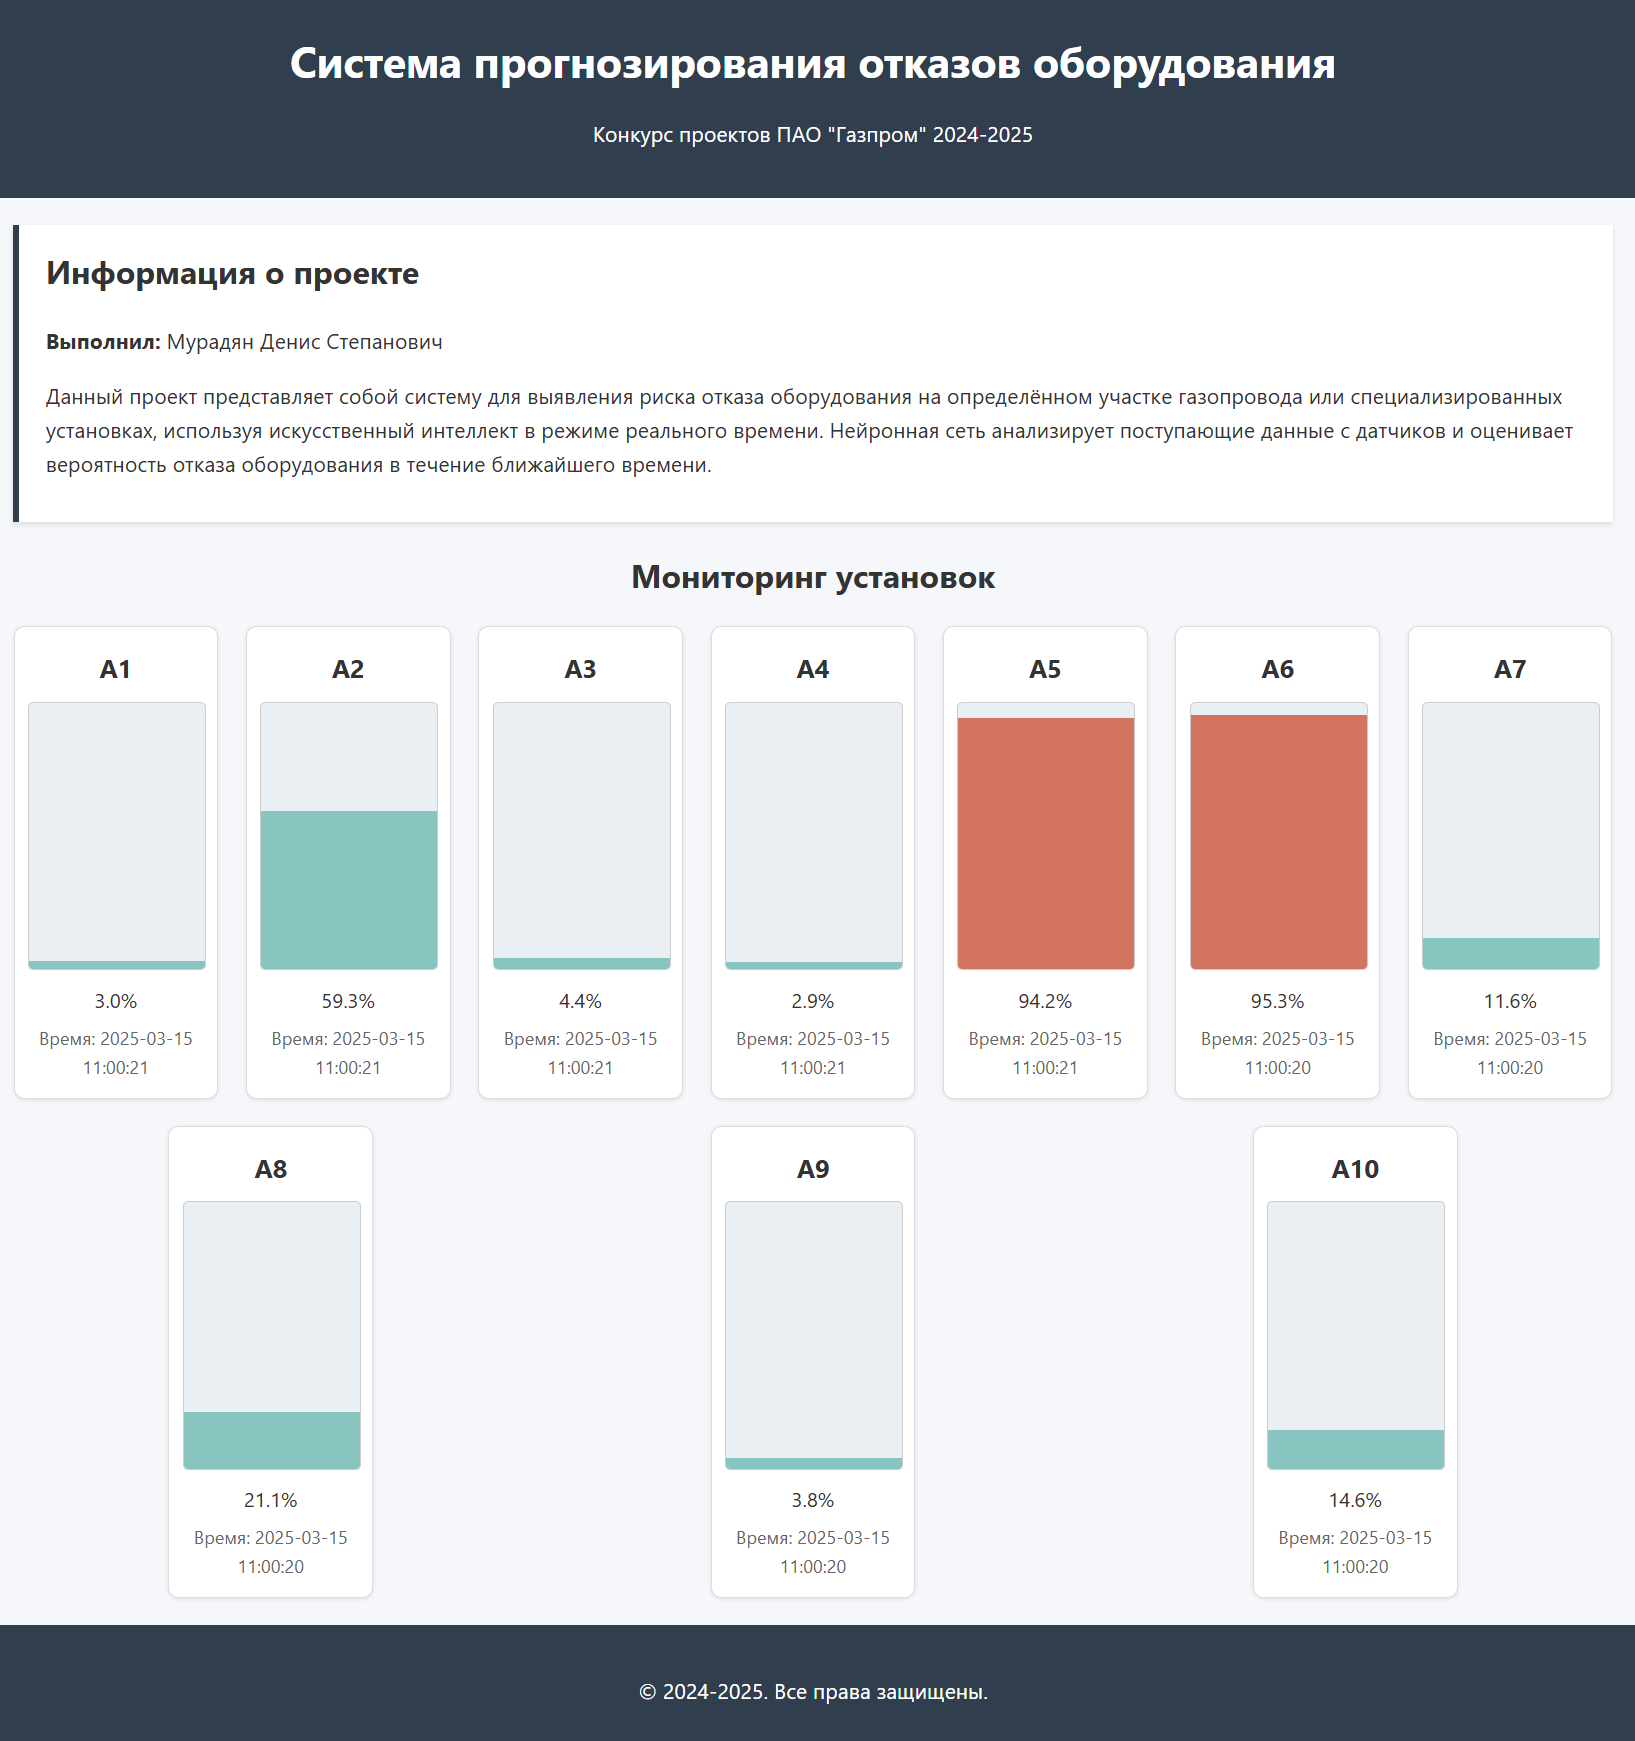
\includegraphics[width=0.7\textwidth]{../Include/dashboard.png}
\end{center}

Разработанная система обладает потенциалом для дальнейшего расширения функциональности.
В перспективе можно добавить возможность отправки оповещений на мобильные устройства,
чтобы пользователи получали мгновенные уведомления в случае достижения критических значений риска.
Такая функциональность позволит оперативно реагировать на опасные ситуации вне зависимости от местонахождения оператора.

Также, реализация проекта позволяет легко интегрировать его в более масштабные информационные системы и экосистему компании.
Таким образом, при дальнейшем расширении, можно внедрить, к примеру, такую функцию: при достижении установкой
«красной зоны» риска, система может автоматически инициировать уменьшение темпа работы оборудования и вызов сервисной бригады
для диагностики и устранения неисправностей.
Это позволит не только повысить уровень безопасности, но и оптимизировать производственные процессы, снижая потенциальные убытки.

Стабильная работа проекта, удобный интерфейс и перспективы дальнейшего расширения свидетельствуют о
высокой готовности решения к внедрению в реальных условиях эксплуатации.

\section{Заключение}

Данный проект представляет собой высокотехнологичное и инновационное решение для мониторинга и прогнозирования
отказов оборудования, основанное на анализе данных в реальном времени. Применение искусственного интеллекта,
а именно GRU-модели обеспечивает исключительную точность предсказаний, позволяя оперативно выявлять риски и
предотвращать аварийные ситуации. Искусственная генерация датасетов демонстрирует работоспособность системы в условиях,
максимально приближенных к реальности. Получение данных через REST API обеспечивает быструю и эффективную интеграцию
системы в инфраструктуру предприятия. Это решение не только существенно повышает безопасность эксплуатации объектов,
но и способствует экономической эффективности, снижая затраты на ремонт и минимизируя экологические риски.
Внедрение данного проекта является значимым шагом в развитии интеллектуальных систем управления оборудованием,
отвечая актуальным требованиям современного производства и обеспечивая надежную защиту критически важных объектов.
\end{flushleft}


\end{document}
